    %\subsubsection{VR integration and data visualization interface}
    %\label{subsubsec:VR_integration}
    %%Define the sections of the VR interface and how information is displayed
    %\input{Text/VR_integration}

Finally, the `Virtual reality integration' module, developed in Unity, serves as the third critical component.
This module includes an immersive simulation and a data visualization interface that transports users into the VR simulation of the experiment's location for facade complexity analysis.

Within this dynamic virtual environment, participants can explore and interact with the building from both inside and outside, visualize its context, and manipulate the facade variations through the user interface.

Seamlessly integrated with the simulation, the interface provides real-time feedback on the impact of different facade variations on the building, facilitating more effective and informed decision-making when selecting a specific level of complexity.

    %% Figure of Real building next to VR
     \begin{figure}[t]
          \centering
          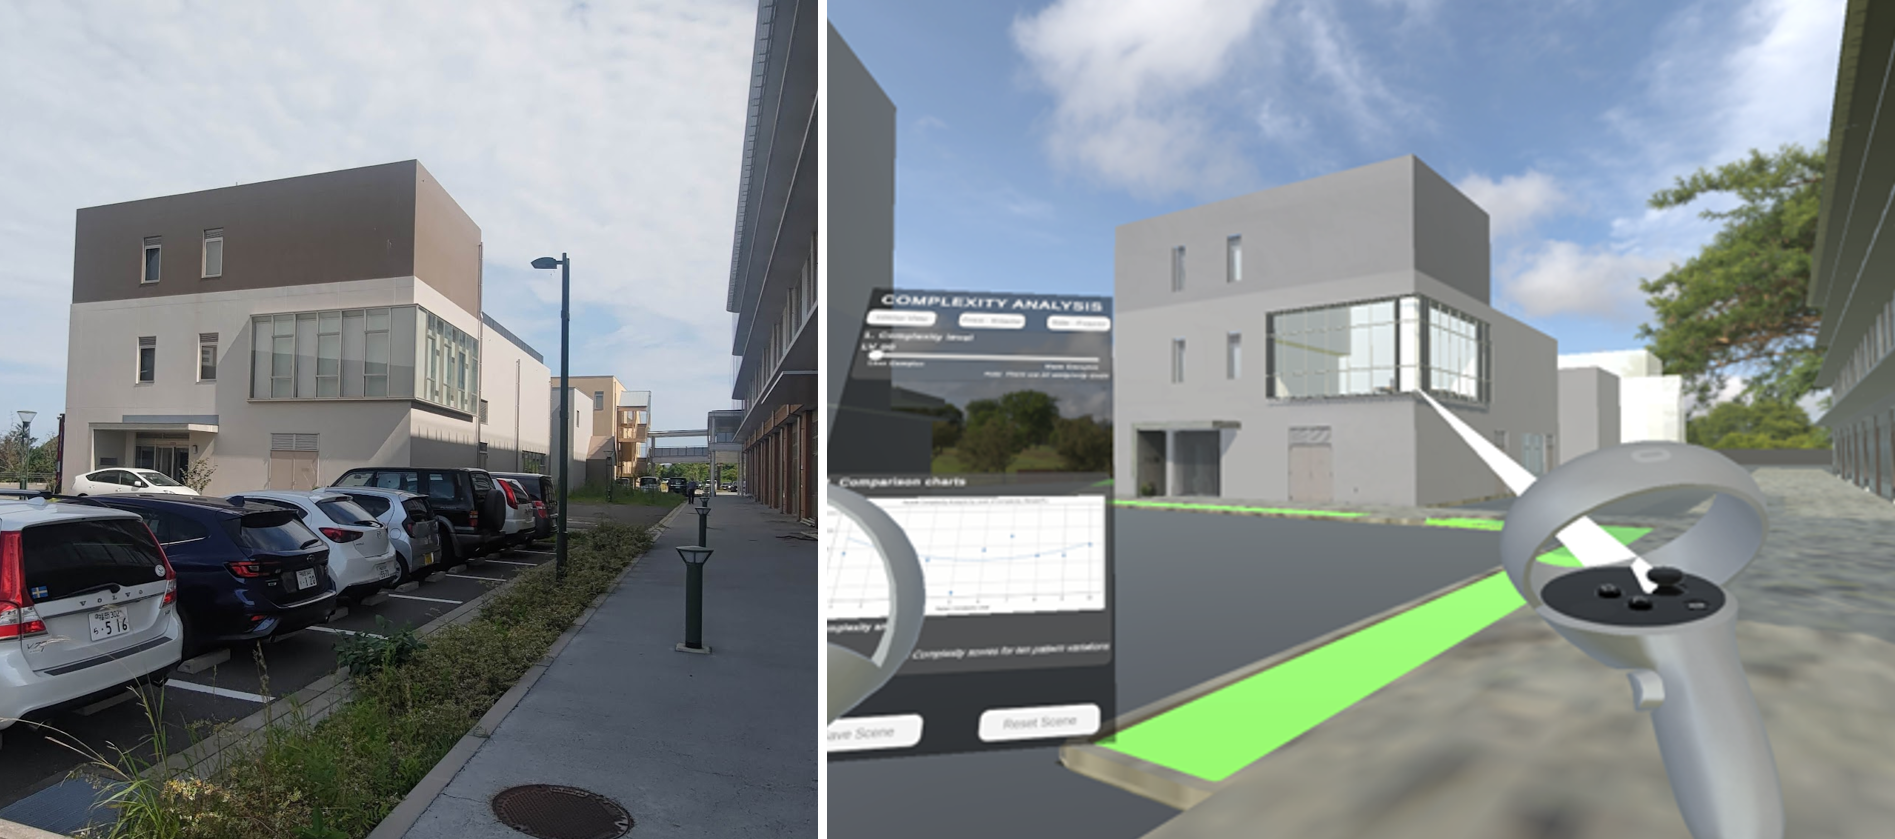
\includegraphics[width= \linewidth]{Images/RealvsVRBuildling}
          \caption{Comparison side by side of actual photography (left) of laboratory building used for experiment and virtual clone (right) modeled and simulated in VR for the Complexity analysis experiment in facade design.}
          \label{fig:RealVsVR}
        \end{figure}

        %% Figure of interior and exterior VR
     \begin{figure}[t]
          \centering
          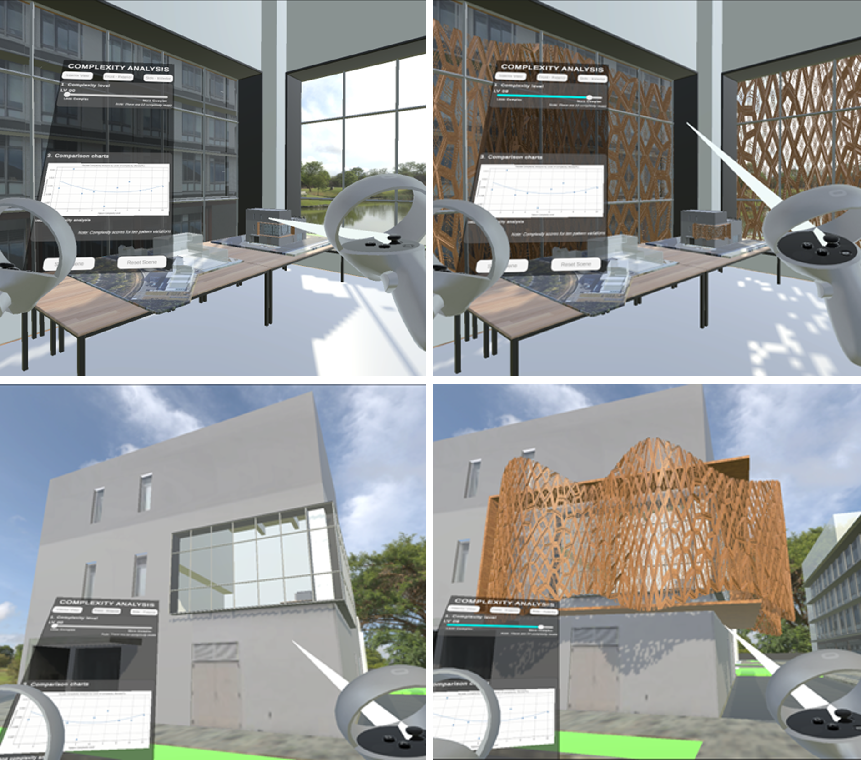
\includegraphics[width= \linewidth]{Images/VRInteriorExterior}
          \caption{VR simulation of interior and exterior of existing building at Kyushu University. (Left) Simulation of current building and (Right) simulation of Complex façade variation.}
          \label{fig:VRInteriorExterior}
        \end{figure}

       %% Figure of interior and exterior VR
     \begin{figure}[htb]
          \centering
          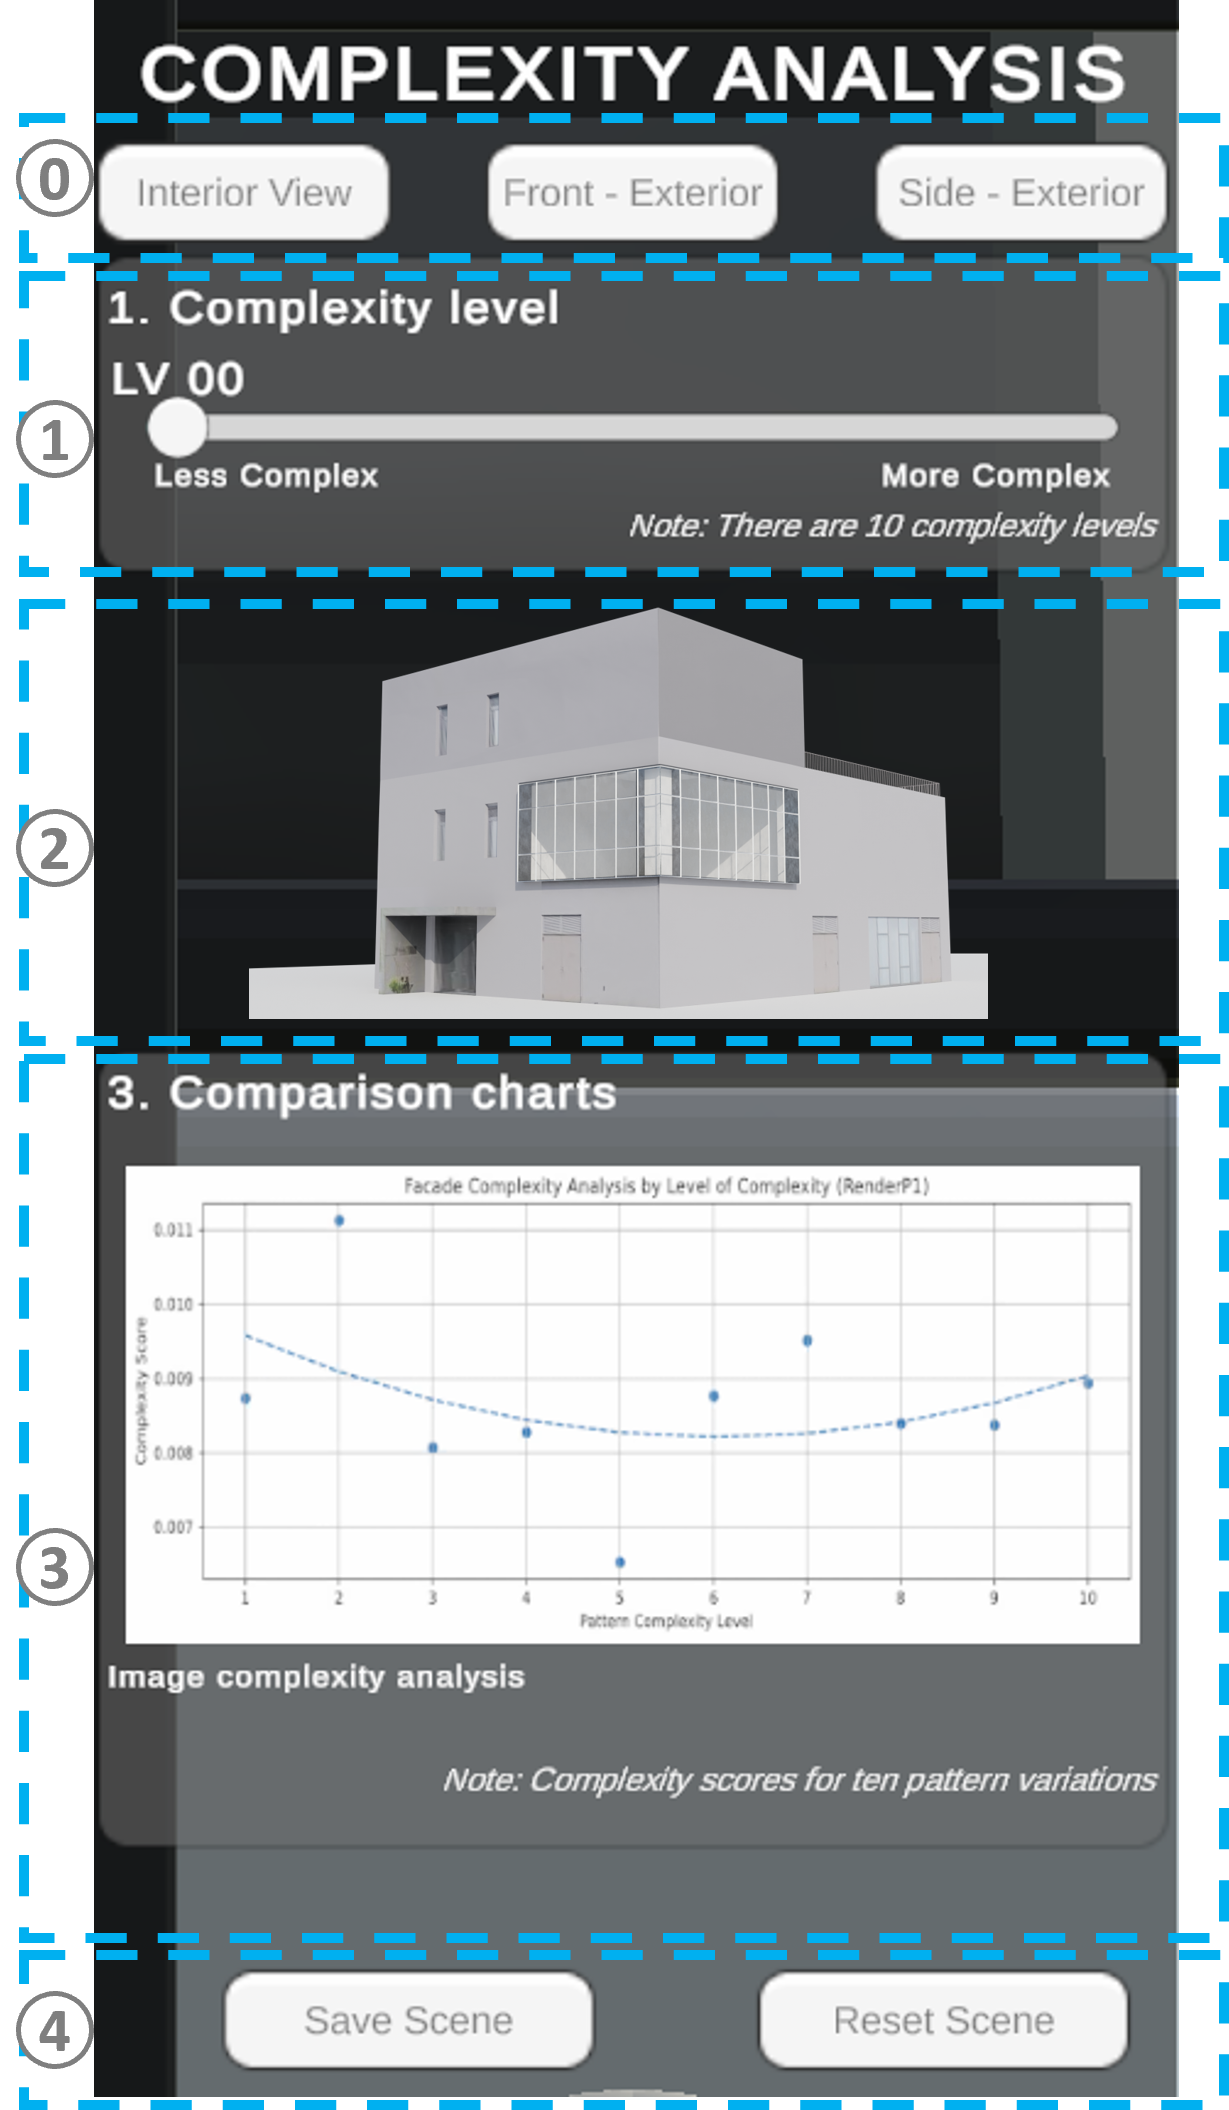
\includegraphics[width= \linewidth]{Images/VRInterface}
          \caption{VR interface for complexity tolerance analysis in facade design. 0) Predetermined cameras, 1) Slider with ranking of levels of complexity, 2) Render preview of facade design, 3) Comparison scatter graph with complexity scores per level of complexity, 4) Save and reset buttons also used to transition among the three patterns.}
          \label{fig:VRInterface}
        \end{figure}